\section{Graph Convolution Networks}
In a GCN the neighbour embeddings are normalized and summed. These embeddings are then transformed using a weight matrix and a non linear function is applied. See Figure \ref{GCN} (page \pageref{GCN}).
\begin{figure}
     \centering
     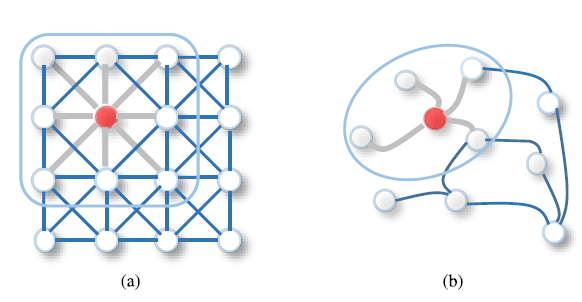
\includegraphics[width= 0.6\textwidth]{pics/GNN.png}
     \caption{2D convolution vs Graph Convolution}
     \label{GCN}
     %add_ref
\end{figure}

\begin{displaymath}
    h_u^{(k)} = \sigma \left( W^{(k)} \sum_{v \in N(u) \cup \{u\}} \frac{h_v}{\sqrt{|N(u)||N(v)|}}\right)
\end{displaymath}

This can be expressed in matrix representation as
\begin{displaymath}
    x*_{G} g{\theta} =\theta(I_{n}+D^{-\frac{1}{2}}AD^{-\frac{1}{2}})x
\end{displaymath}
where D is diagonal degree matrix, A is adjacency matrix and x is the input

An example of nodes in a graph and their adjacency matrix is shown in Figure \ref{example_graph} (page \pageref{example_graph}).

\begin{displaymath}
    A = {\begin{bmatrix}
0 & 1 & 1\\
0 & 0 & 1\\
0 & 0 & 0
\end{bmatrix}}, N = {\begin{bmatrix}
    a \\ b \\c
\end{bmatrix}}, A^T.N = {\begin{bmatrix}
    0 \\ a \\ a+b
\end{bmatrix}}
\end{displaymath}

\begin{figure}
    \centering

\begin{tikzpicture}
\tikzset{% This is the style settings for nodes
    dep/.style={circle,minimum size=1cm,fill=orange!20,draw=orange,
                general shadow={fill=gray!60,shadow xshift=1pt,shadow yshift=-1pt}},
    cli/.style={circle,minimum size=1cm,fill=white,draw,
                general shadow={fill=gray!60,shadow xshift=1pt,shadow yshift=-1pt}},
    spl/.style={cli,append after command={
                  node[circle,draw,dotted,
                       minimum size=1.5cm] at (\tikzlastnode.center) {}}},
    c1/.style={-stealth,very thick,red!80!black},
    v2/.style={-stealth,very thick,yellow!65!black},
    v4/.style={-stealth,very thick,purple!70!black}}
\node[cli] (0) at (0,0) {a};
\node[cli] (1) at (-1,-2) {b};
\node[cli] (2) at (2,-2) {c};
%\draw[c1] (0) to[bend right] (7);
\draw[v4] (0) -- (1);
\draw[v4] (0) -- (2);
\draw[v4] (1) -- (2);
\end{tikzpicture}


    \caption{Example Graph}
    \label{example_graph}
\end{figure}

